\chapter{Implementation}
\label{cha:Implementation}

\section{Generalising the Codebase}
\label{sec:Generalising the Codebase}
The simulators created for this project were created partly using the AIM simulator codebase \citep{AIMWebsite}. We wanted to expand the simulator so that it could run AV simulations in situations other than 4-way intersections. To do this we needed to generalise the AIM codebase so that new developers could add simulators with very little effort, however, we also needed to ensure that these changes would not affect the functionality of the AIM simulator. These changes to the codebase were done in conjunction with Rebecca Milligan, who is also working on AV simulations in her car park management project.

To generalise the codebase we refactored key classes into separate general and AIM specific classes. The general classes can be expanded to create other simulator specific classes, whilst the AIM specific classes maintain the functionality of the original simulator. This helps to reduce code duplication when developing new simulators.

All class diagrams were created using IntelliJ IDEA 15.0.3 internal diagram tool. Figure \ref

\includegraphics[width=\textwidth]{}

\subsection{aim4.driver}
\label{subsec:aim4.driver}
\emph{aim4.driver} controls how a vehicle behaves on the map. In the original simulator the drivers were built to deal with 4-way intersections, with general functionality tied into the same class. You can see how this was done in Figures \ref{fig:driverBefore} and \ref{fig:driverAfter}.

\begin{figure}[htb]
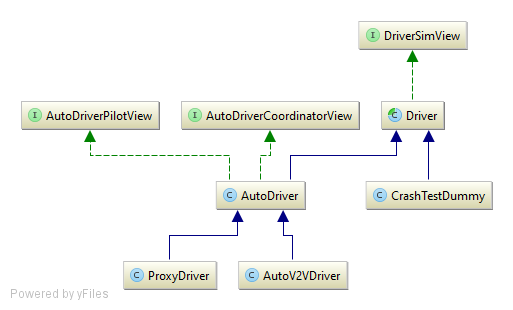
\includegraphics[width=\textwidth]{classDiagrams/driverBefore.png}
\caption{The original class structure for \emph{Driver}.}
\label{fig:driverBefore}
\end{figure}

\begin{figure}[htb]
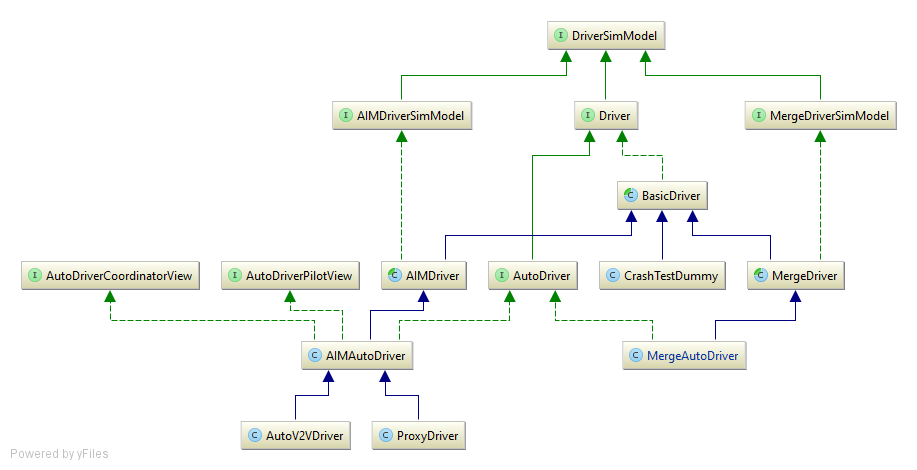
\includegraphics[width=\textwidth]{classDiagrams/driverAfter.png}
\caption{The new class structure for \emph{Driver}.}
\label{fig:driverAfter}
\end{figure}

The first major change was renaming \emph{DriverSimView}, \emph{AutoDriverPilotView}, and \emph{AutoDriverCoordinatorView} to end in \emph{Model} instead of \emph{View}. These interfaces are used to limit the methods that other classes can access in Driver and AutoDriver, thus changing their 'view' of that class. We felt that \emph{View} could cause confusion with the GUI elements of the simulator; we instead chose to refer to these interfaces as \emph{Models}, because the accessors are effectively given a model of Driver and AutoDriver (beyond which they care very little) that they can use to access methods.

The next change was separating out all of the AIM specific code into its own classes and interfaces. You can see how this was done in Figure \ref{fig:driverAfter} with \emph{AIMDriverSimModel} and \emph{AIMDriver}. The merge specific code found in \emph{MergeDriverSimModel}, \emph{MergeDriver} and \emph{MergeAutoDriver} is structured in a very similar manner to its AIM counterpart, taking advantage of the generalised code.

As a consequence of breaking out the code like this, a number of additional changes had to be made. Driver was changed into an interface and a new class \emph{BasicDriver}. \emph{Driver} is simply used as an interface for accessing Drivers in non-simulation contexts (such as \emph{BasicVehicle}). \emph{BasicDriver} contains the generalised functionality all \emph{Driver} objects should need, with AIM specific activities moved to \emph{AIMDriver}. Extending from \emph{Driver} is the \emph{AutoDriver} interface, which adds no new methods but is instead used to categorise autonomous drivers. \emph{AIMAutoDriver} contains almost exactly the same code as the original \emph{AutoDriver} class.

\subsection{aim4.gui}
\label{subsec:aim4.gui}
\emph{aim4.gui} controls the GUI for the simulator. We had to adjust this to allow for non-AIM simulations to be run. We chose to use tabs to allow users to switch between simulators (these are greyed out when a simulation is running). To make adding new tabs and simulation screens easier we had to refactor \emph{Viewer} into smaller, separate components. You can see the structural changes in Figures \ref{fig:originalAIMSetupLabeled} and \ref{fig:newAIMSetupLabeled}.

\begin{figure}[htb]
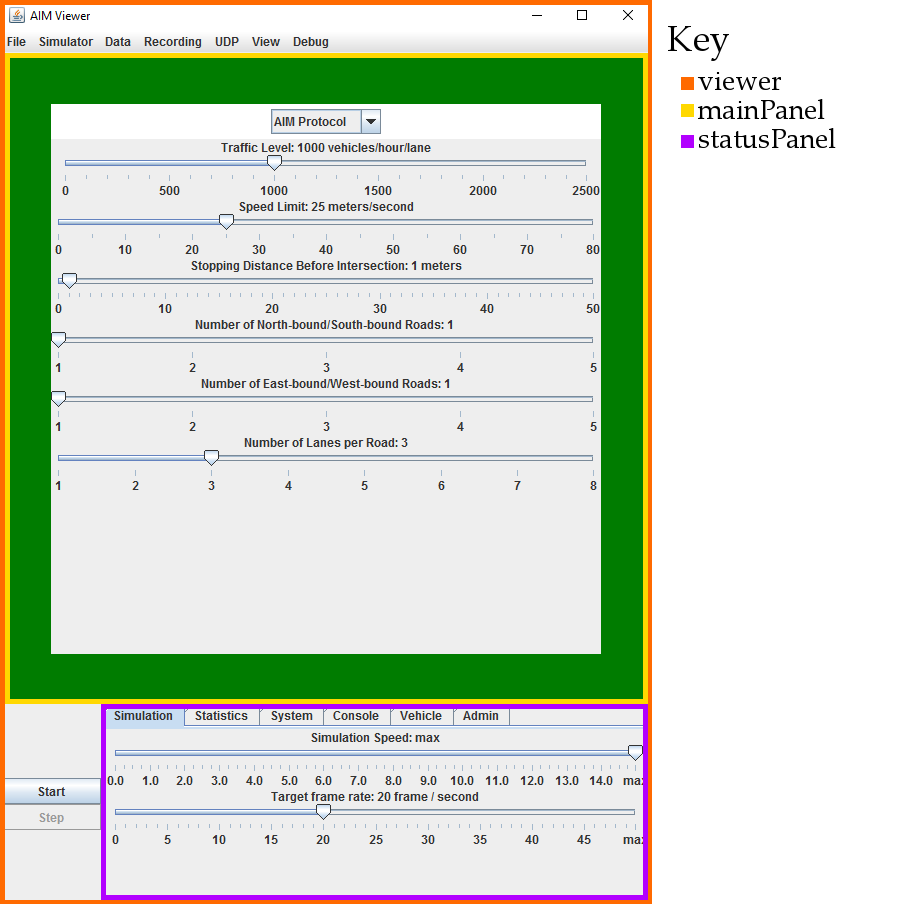
\includegraphics[width=\textwidth]{screenshots/originalAIMSetupLabeled.png}
\caption{Panel layout in the original simulator.}
\label{fig:originalAIMSetupLabeled}
\end{figure}

\begin{figure}[htb]
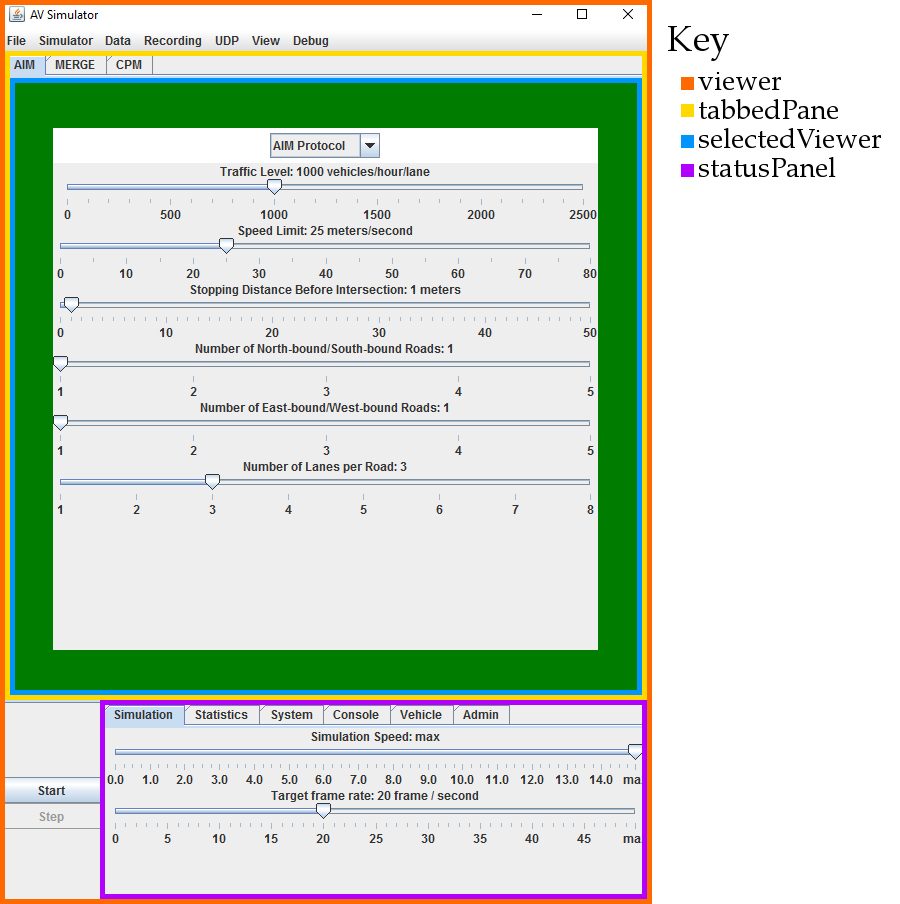
\includegraphics[width=\textwidth]{screenshots/newAIMSetupLabeled.png}
\caption{Panel layout in the new simulator.}
\label{fig:newAIMSetupLabeled}
\end{figure}

In the original simulator \emph{Viewer} displays the simulator set-up controls, \emph{SimSetupPanel}, and the simulation viewer \emph{Canvas} inside \emph{mainPanel}. \emph{mainPanel} is a \emph{JPanel} with a \emph{CardLayout} allowing the panel to switch between displaying the set-up controls and the viewer. In the new simulator we replaced \emph{mainPanel} with \emph{tabbedPane}, a \emph{JTabbedPane} object that allows users to switch between the different simulators using tabs. Each tab displays a \emph{SimViewer}, which behaves in a similar way to \emph{mainPanel} allowing users to switch between the set-up screen and the simulation screen using \emph{CardLayout}. Each simulator will have their own SimViewer type, as shown in Figure \ref{fig:simViewer}.

\begin{figure}[htb]
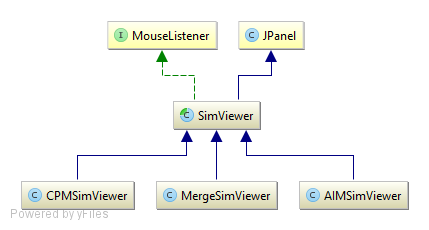
\includegraphics[width=\textwidth]{classDiagrams/simViewer.png}
\caption{The class diagram for \emph{SimViewer}.}
\label{fig:simViewer}
\end{figure}

We didn't want to force new simulators to use a full representation of vehicles on screen, as \emph{Canvas} does. To avoid this we created a new interface \emph{SimScreen} which \emph{SimViewer} uses to describe it's viewer card. Any class implementing \emph{SimScreen} can be used as the viewer for a simulation. Figure \ref{fig:simScreen} shows how \emph{MergeStatScreen} and \emph{Canvas} using \emph{SimScreen}.

\begin{figure}[htb]
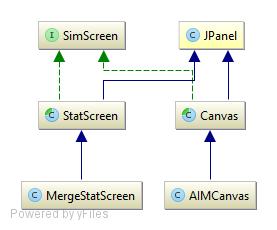
\includegraphics[width=\textwidth]{classDiagrams/simScreen.png}
\caption{The class diagram for \emph{SimScreen}.}
\label{fig:simScreen}
\end{figure}

We also generalised the \emph{SimSetupPanel} class to allow \emph{SimViewer} to display non-AIM set-up controls. Figure \ref{fig:simSetupPanel} shows the new class structure for \emph{SimSetupPanel}.

\begin{figure}[htb]
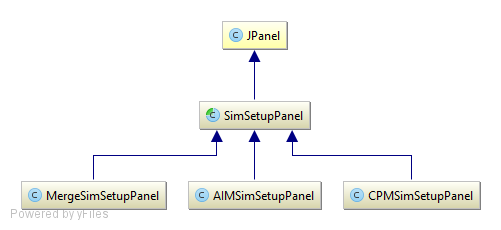
\includegraphics[width=\textwidth]{classDiagrams/simSetupPanel.png}
\caption{The class diagram for \emph{SimSetupPanel}.}
\label{fig:simSetupPanel}
\end{figure}

We also made a small adjustment to the behaviour of the reset option in the menu. Now the simulator must be paused in order for the reset button to be active. We did this because resetting the simulator without pausing was creating \emph{NullPointerException}s.

\subsection{aim4.map}
\label{subsec:aim4.map}
\emph{aim4.map} is used to describe the environment vehicles are required to navigate. They also spawn vehicles that then drive through the map. Figures \ref{fig:mapBefore} and \ref{fig:mapAfter} show the original and new class structure for \emph{aim4.map}.

\begin{figure}[htb]
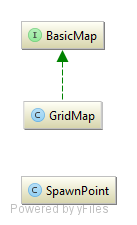
\includegraphics[width=\textwidth]{classDiagrams/mapBefore.png}
\caption{The original class structure for \emph{BasicMap} and \emph{SpawnPoint}.}
\label{fig:mapBefore}
\end{figure}

\begin{figure}[htb]
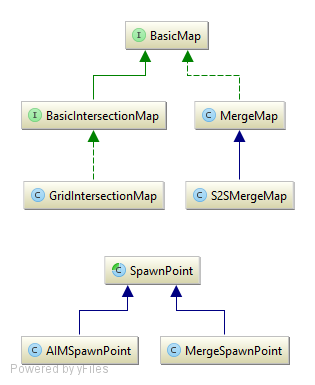
\includegraphics[width=\textwidth]{classDiagrams/mapAfter.png}
\caption{The new class structure for \emph{BasicMap} and \emph{SpawnPoint}.}
\label{fig:mapAfter}
\end{figure}

The changes made to \emph{aim4.map} were relatively straight-forward. The AIM specific features in \emph{BasicMap} were extracted out in \emph{BasicIntersectionMap} and \emph{GridMap} was renamed to \emph{GridIntersectionMap} and now inherits from the new interface. This allows for new map types, such as \emph{MergeMap} to implement a map type without AIM features.

\emph{SpawnPoint} was also broken out into general and AIM specific features. This had to be done because \emph{SpawnPoint} used to create \emph{SpawnSpec} objects with \emph{destination} fields. \emph{destination} is an AIM specific field relating to the intersection exit a vehicle plans to reach. By extracting this out new map types can spawn vehicles with \emph{SpawnSpec} instances specific to their map type.

\subsection{aim4.sim}
\label{subsec:aim4.sim}
\emph{aim4.sim} contains the code responsible for constructing and running simulations. The original code was very focussed on AIM simulations and so we had to break the interfaces to allow for different types of simulators. 

\emph{Simulator} is an interface that new simulators need to implement. We decided to extract out some of the AIM specific features into \emph{AIMSimulator}. We also added an override to \emph{getMap()}, forcing AIM simulators to use \emph{BasicIntersectionMap} maps. The class structure changes can be seen in Figures \ref{fig:simulatorBefore} and \ref{fig:simulatorAfter}.

\begin{figure}[htb]
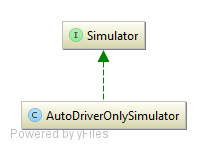
\includegraphics[width=\textwidth]{classDiagrams/simulatorBefore.png}
\caption{The original class structure for \emph{Simulator}.}
\label{fig:simulatorBefore}
\end{figure}

\begin{figure}[htb]
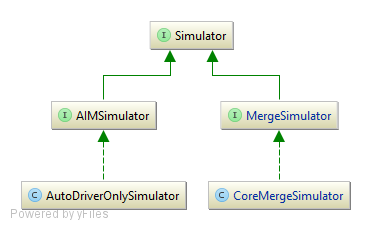
\includegraphics[width=\textwidth]{classDiagrams/simulatorAfter.png}
\caption{The new class structure for \emph{Simulator}.}
\label{fig:simulatorAfter}
\end{figure}

\emph{SimSetup} was also modified to separate AIM specific set-up options and simulator creation code from other simulators. Figures \ref{fig:simSetupBefore} and \ref{fig:simSetupAfter} show how these classes were altered.

\begin{figure}[htb]
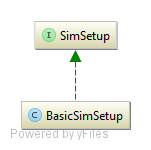
\includegraphics[width=\textwidth]{classDiagrams/simSetupBefore.png}
\caption{The original class structure for \emph{SimSetup}.}
\label{fig:simSetupBefore}
\end{figure}

\begin{figure}[htb]
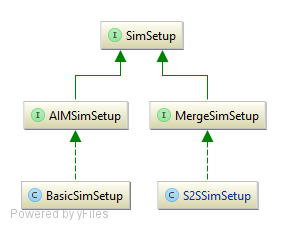
\includegraphics[width=\textwidth]{classDiagrams/simSetupAfter.png}
\caption{The new class structure for \emph{SimSetup}.}
\label{fig:simSetupAfter}
\end{figure}

\subsection{aim4.vehicle}
\label{subsec:aim4.vehicle}
\emph{aim4.vehicle} controls the different vehicles used during simulations. Vehicles are used by both \emph{Driver} and \emph{Simulator} instances. To allow them to do that the original simulator code used \emph{View} interfaces similar to those in \ref{subsec:aim4.driver}. Figure \ref{fig:vehicleBefore} shows how these interfaces link together. Extracting AIM behaviour was quite difficult because of how interconnected these interfaces were. The solution we came up with was to create AIM specific interfaces and link them together in a similar manner, inheriting from the generic ones if possible. Figure \ref{fig:vehicleAfter} shows how the new structure links together.

\begin{figure}[htb]
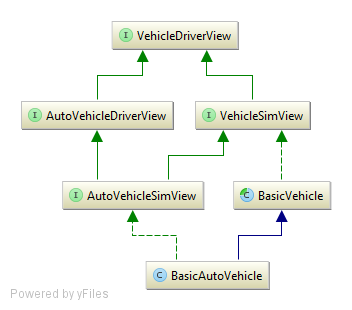
\includegraphics[width=\textwidth]{classDiagrams/vehicleBefore.png}
\caption{The original class structure for \emph{aim4.vehicle}.}
\label{fig:vehicleBefore}
\end{figure}

\begin{figure}[htb]
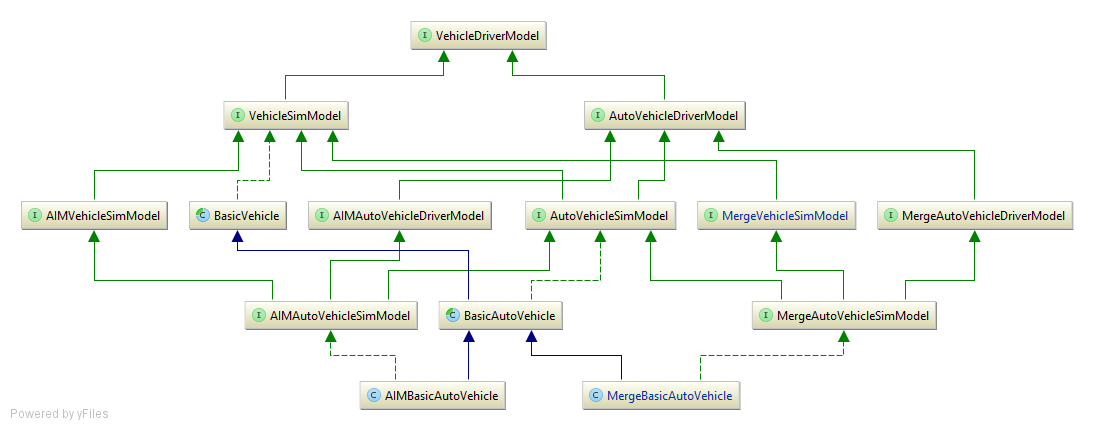
\includegraphics[width=\textwidth]{classDiagrams/vehicleAfter.png}
\caption{The new class structure for \emph{aim4.vehicle}.}
\label{fig:vehicleAfter}
\end{figure}

The first change made to \emph{aim4.vehicle} was to rename all of the files ending in \emph{View} to end in \emph{Model} instead. This matches the changes made to \emph{aim4.driver}.

\emph{AIMVehicleSimModel} and \emph{AIMAutoVehicleDriverModel} are at the top of the AIM interface tree. They both extend their generic counterparts. \emph{AIMAutoVehicleSimModel} extends these two interfaces along with \emph{AutoVehicleSimModel}. This matches up to the original inheritance structure. Any future vehicles will need to create their own version of these interfaces, as seen in \emph{MergeVehicleSimModel}, \emph{MergeAutoVehicleDriverModel} and \emph{MergeAutoVehicleSimModel}. 

In terms of classes we made \emph{BasicAutoVehicle} abstract and extracted out AIM specific behaviour to \emph{AIMBasicAutoVehicle}. \emph{BasicAutoVehicle} had to be abstract because we wanted to force \emph{getDriver()} to be overridden in subclasses to retrieve the simulator specific \emph{AutoDriver} for that vehicle (for example \emph{AIMAutoDriver} in AIM simulators). 


